At the end of this worksheet you should be able to  
\begin{itemize}
	\item use the properties of waves to solve for an unknown quantity.
	\item use the mathematical description of a wave to plot waves motion over time.
	\item use the conditions of a standing wave on a string to solve for an unknown quantity.
\end{itemize}


\begin{enumerate}
	\setlength\itemsep{2 in}
	
	\item
	The speed of a wave on a string is proportional to the square root of the tension $F$ in the string and the length $L$, and inversely proportional to the square root the mass $m$ of the string.
	\begin{itemize}
		\setlength\itemsep{1 in}
		\item By what factor does the velocity of the wave change if the tension doubles?
		\item What about if the length halves?
		\item What if the mass triples?
		\item What if the mass density doubles?
		\item If the force doubles and the length triples, by what factor does the velocity change?
		\item What if the mass density triples and the force doubles?
		\item By what factor does the force need to change to double the velocity?
		\item By what factor does the length need to change to double the velocity?
		\item By what factor does the length need to change to quarter the velocity? 
		\item If the velocity doubles and the length halves, by what factor does the force need to change?
	\end{itemize}
	
	\item
	A string is \SI{2}{m} long and has a mass of \SI{10}{g}. What is its mass density? If you cut the string in half, what is its mass density then? If you exerted a force of \SI{10}{N}, then what is the velocity of waves on the string? What would the force need to be to make the velocity \SI{100}{m/s}? 
	
	\item
	A string with a mass density of \SI{10}{g/m} has a tension of \SI{100}{N}. A periodic waveform that has a period of \SI{0.1}{s} is put into this string. What is the frequency? What is the wavelength of this wave? What is the angular frequency and what is the wavenumber?
	
	\item
	The wavenumber of a wave is \SI{20}{rad/meter}, and the period is \SI{0.1}{seconds}. 
	\begin{itemize}
		\setlength\itemsep{1 in}
		\item What is the frequency, angular frequency, wavelength, and velocity?
		\item If the force on the string that is carrying this wave is \SI{100}{N}, then what is the linear mass density?
		\item If the string is \SI{10}{grams} then what is the length of the string?
	\end{itemize}
	
	\item
	A \SI{1}{meter} long string with a linear mass density of \SI{10}{g/m} is oriented horizontally and a pulley at one end allows a \SI{1}{kg} to hang down and put tension in the string. What is the speed of waves on this string. 
	
	\item 
	The same string from above is hanging vertically from a support with the \SI{1}{kg} mass tied on the end. What is the speed of a wave \emph{near the mass}? What is the speed of a wave \emph{near the top}?
	
	\item
	A wave has a wavelength of \SI{3}{m} and an amplitude of \SI{2}{m}. It travels with a speed of \SI{5}{m/s}. If the wave has its maximum at the horizontal position of \SI{0}{m} when $t=\SI{0}{s}$, then sketch a plot of the wave at this time below:  \\
	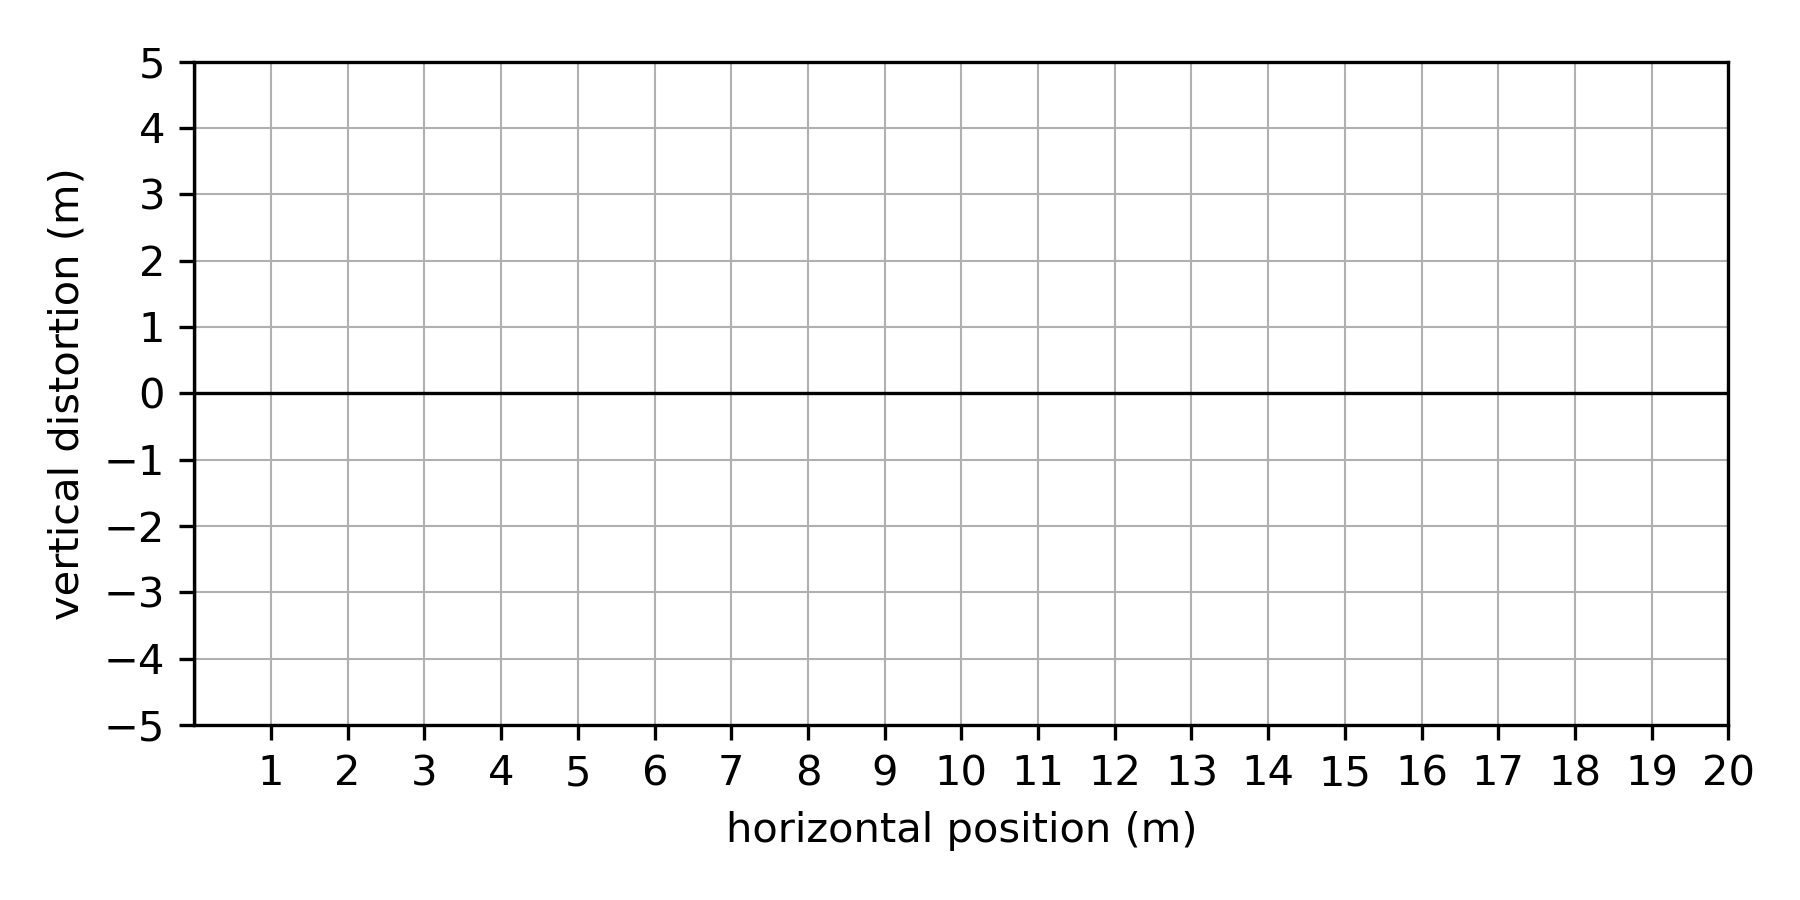
\includegraphics[scale=1]{week13-blank-plot.png}
	
	\item
	Now sketch the wave after \SI{0.2}{seconds} have gone by.\\
	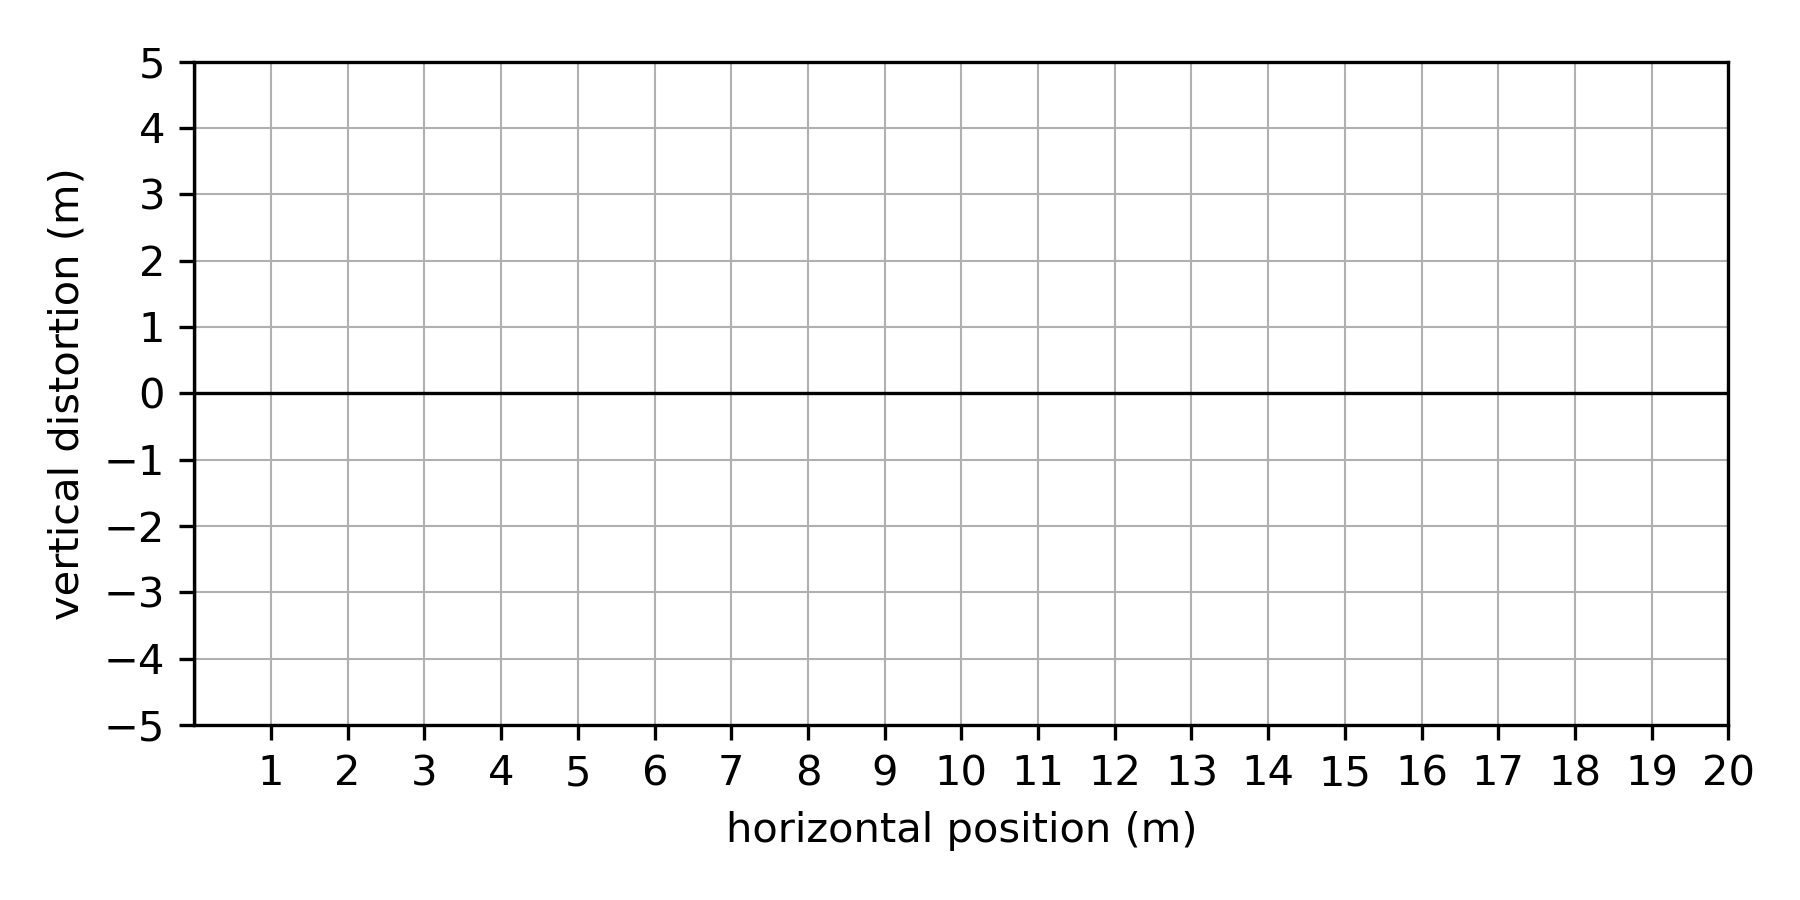
\includegraphics[scale=1]{week13-blank-plot.png}
	
	\item
	Now sketch the wave \SI{1}{second} after the begining.\\
	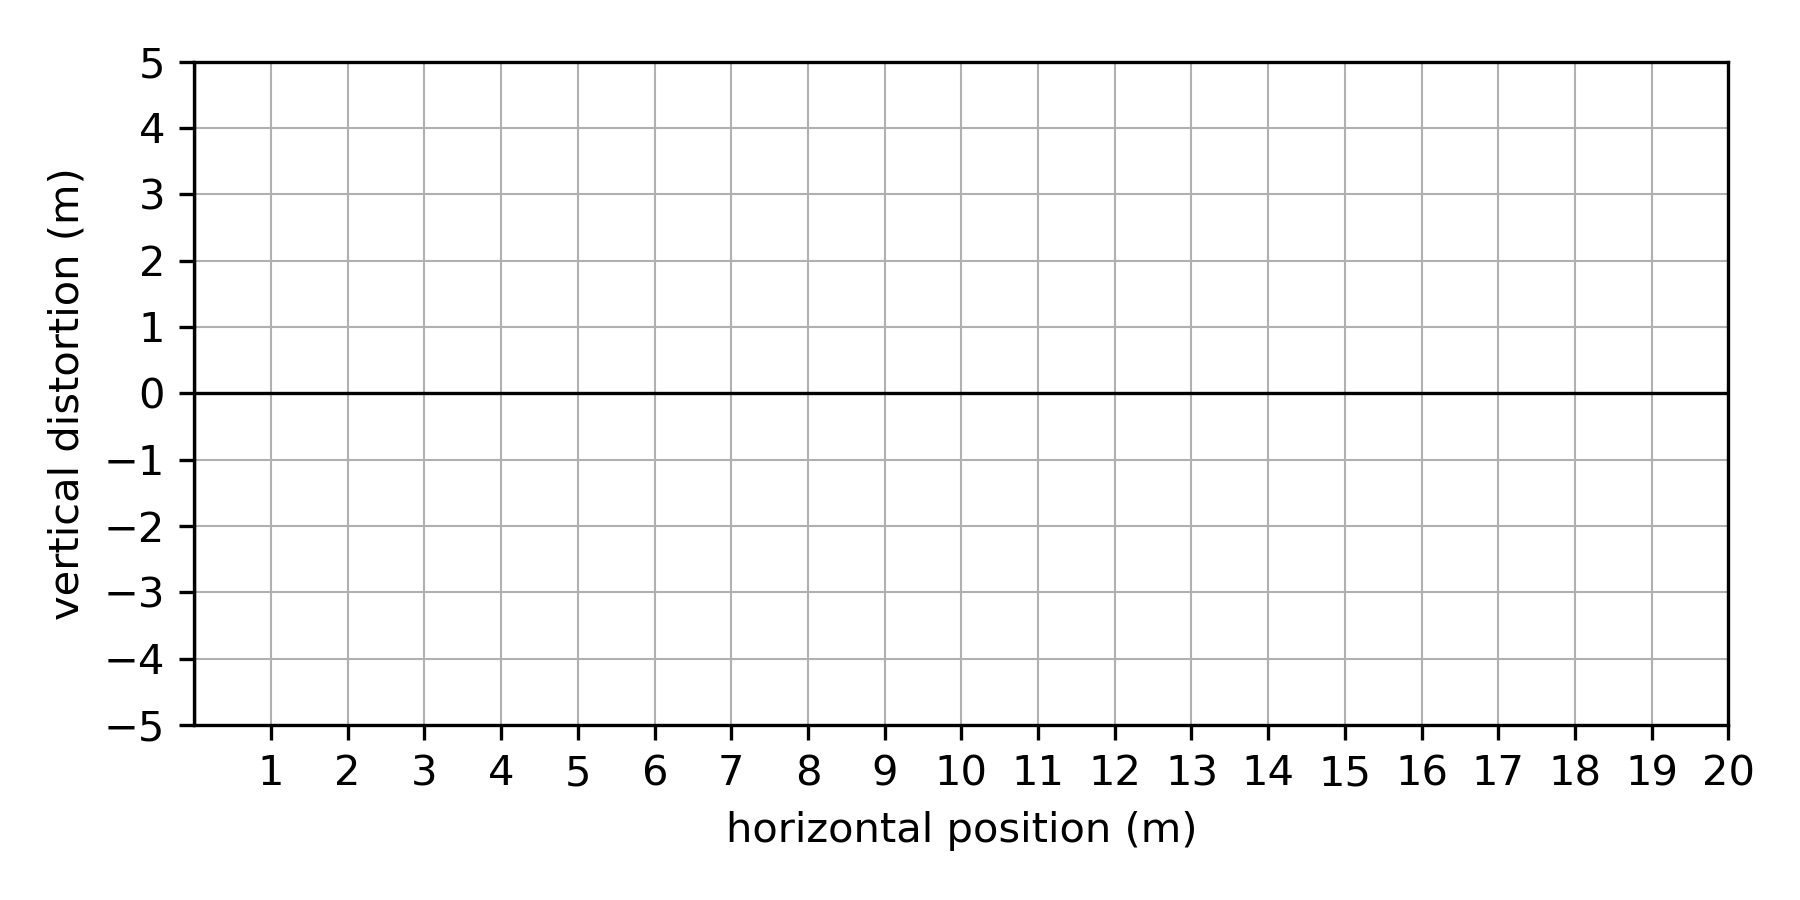
\includegraphics[scale=1]{week13-blank-plot.png}
	
	\item
	The following plot shows a wave at $t=\SI{0}{s}$ and then later when $t=\SI{2}{s}$. What is the wavelength, amplitude, period, angular frequency, wavenumber, and velocity?\\
	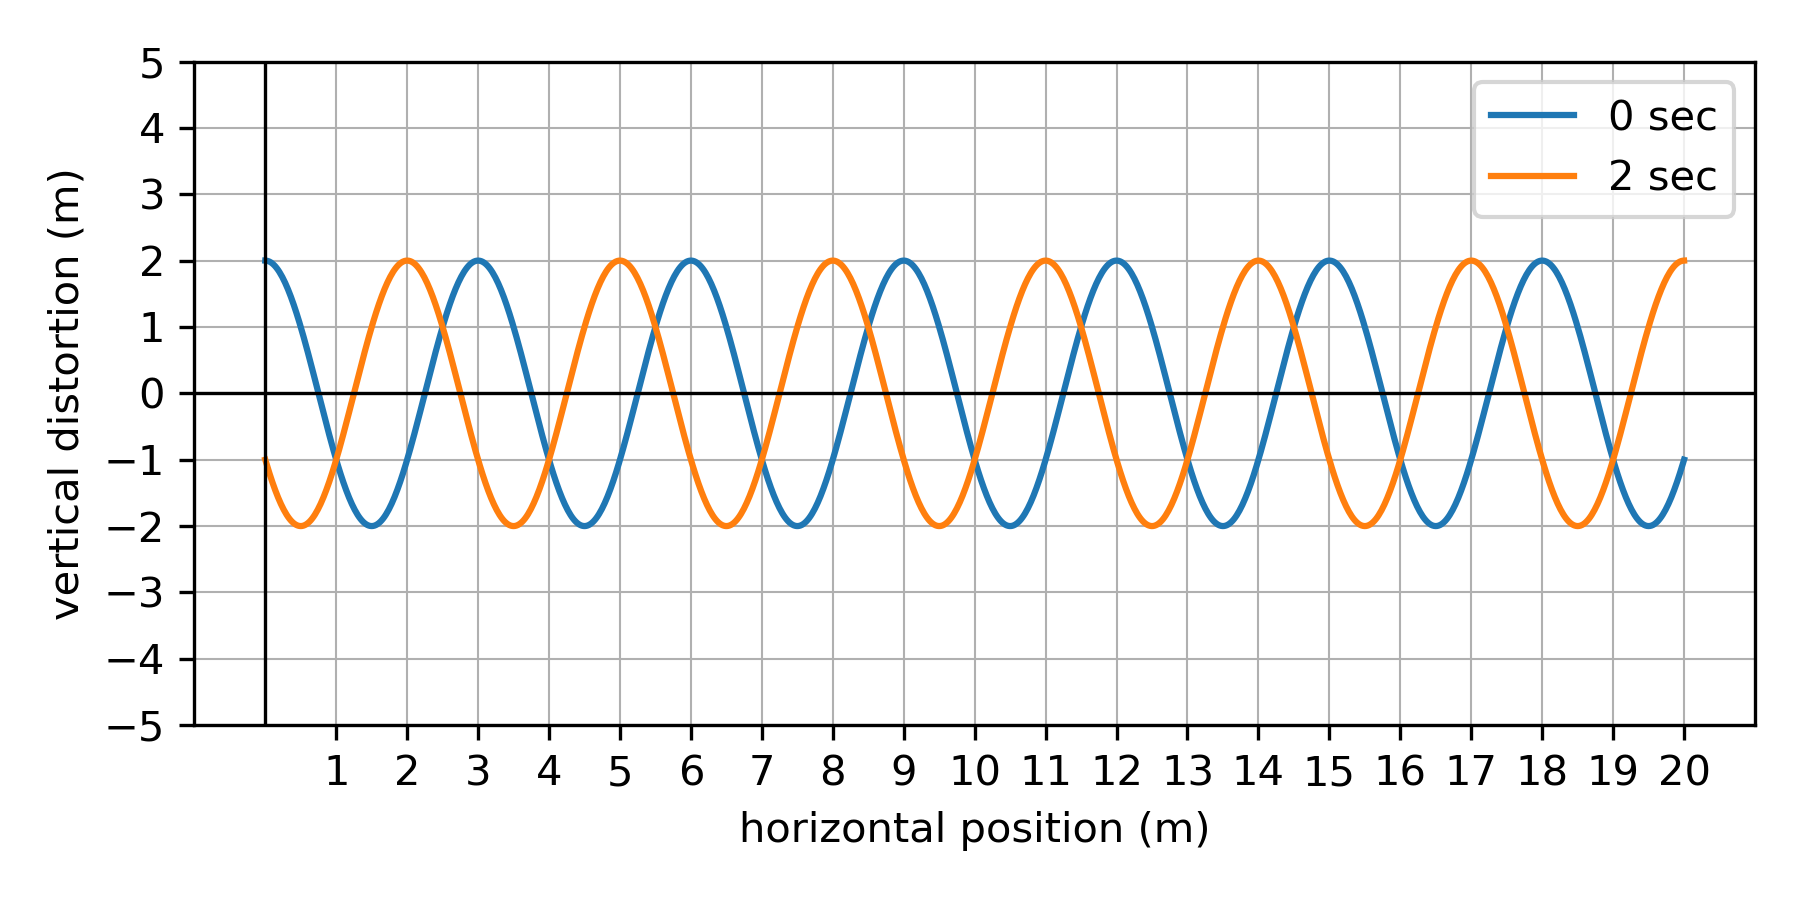
\includegraphics[scale=1]{week13-plot-2-times.png}
	
	\newpage
	\item 
	A wave on a string is described by the equation below. Plot this function for $t=\SI{0}{s}$ and again for $t=\SI{2}{s}$.
	$$y(x,t)=\SI{3.5}{m}\sin\left(\SI{6}{rad/m}\right) x$$%-(\SI{8\pi}{rad/s})t\right)$$
	\\
	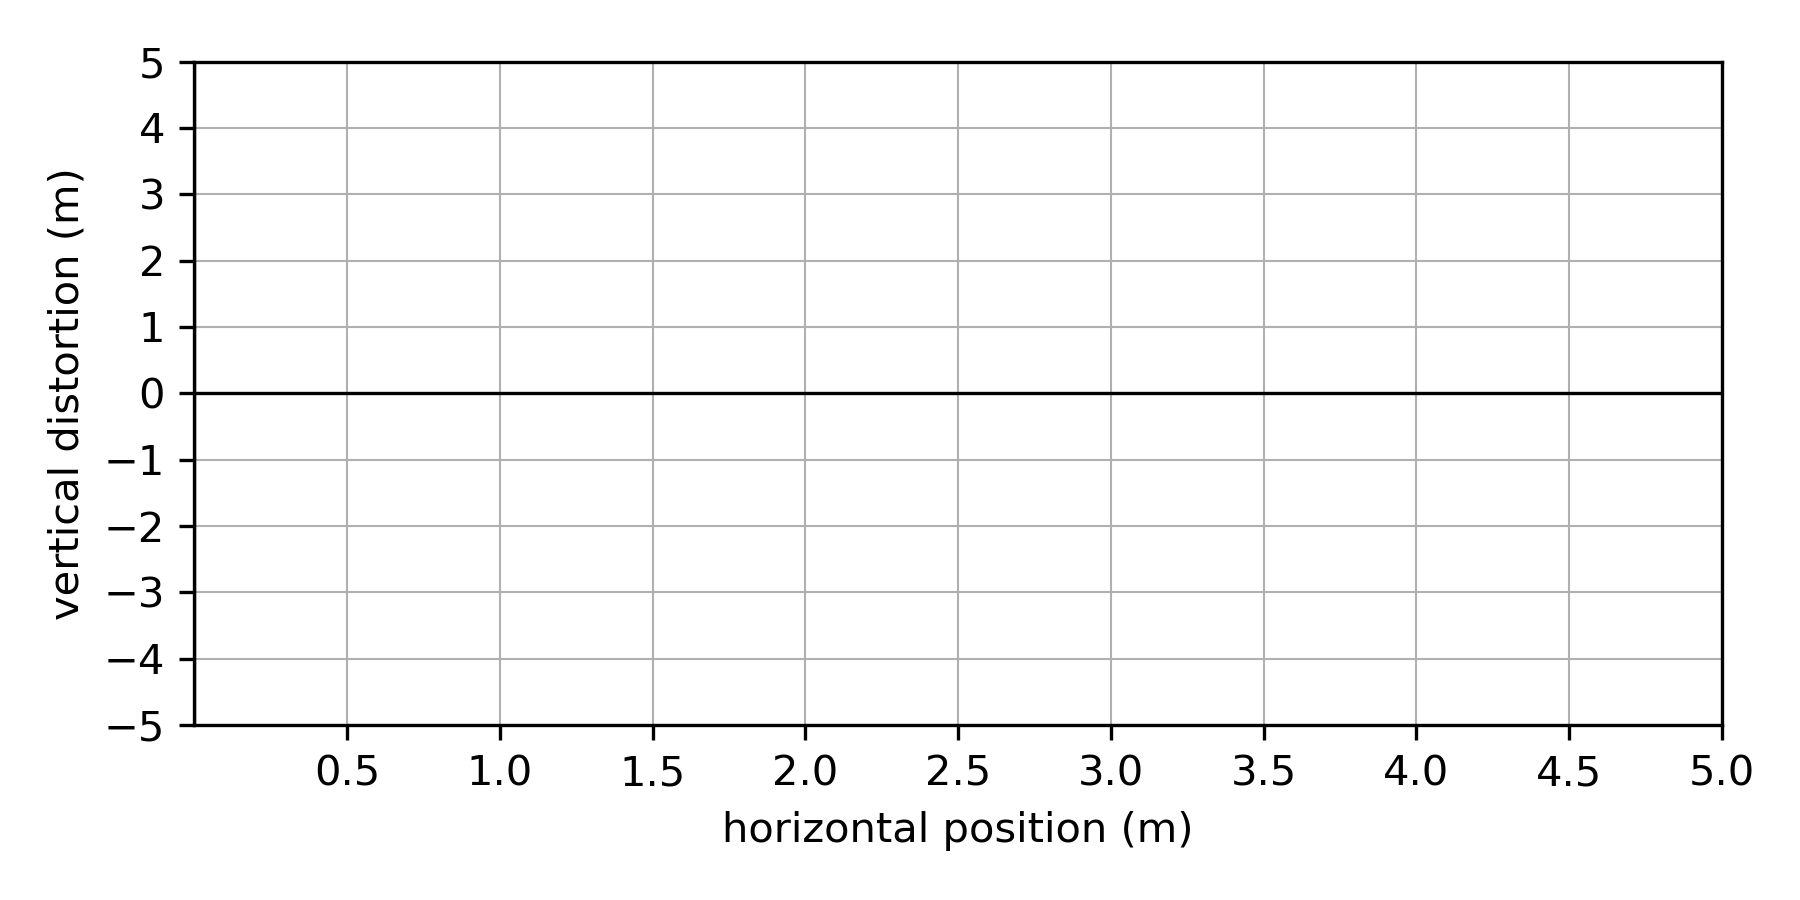
\includegraphics[scale=1]{week13-blank-plot-2.png}
	
	\newpage
	\item
	A string has a tension of \SI{100}{N}. But this string has two sections that are knotted together. One side has a linear mass density of \SI{10}{g/m} and the other side has a linear mass density of \SI{35}{g/m}. What is the velocity of the wave on the first side of the knot? What is the velocity on the second side? If a wave with a wavelength of \SI{0.2}{meters} is traveling on the first side, what is its frequency? When the crest of this wave from the first side reaches the knot, this crest simply passes through the knot. But the velocity has changed. So how much time goes by to when the next crest passes the knot? How far has the first crest traveled in the second side of the string? What does this mean about the wavelength on the second side? What is the frequency of wave crests coming into the knot? What is the frequency of crests leaving the knot? On the basis of this analysis, when the speed of a wave changes suddenly at an interface does the wavelength change or does the frequency or do both change?
	
	\item
	Two waves are approaching each other with speed $v=\SI{4}{m/s}$. At what time and where will these waves fully overlap (their max peaks line up) and what will the wave look like at that time?\\
	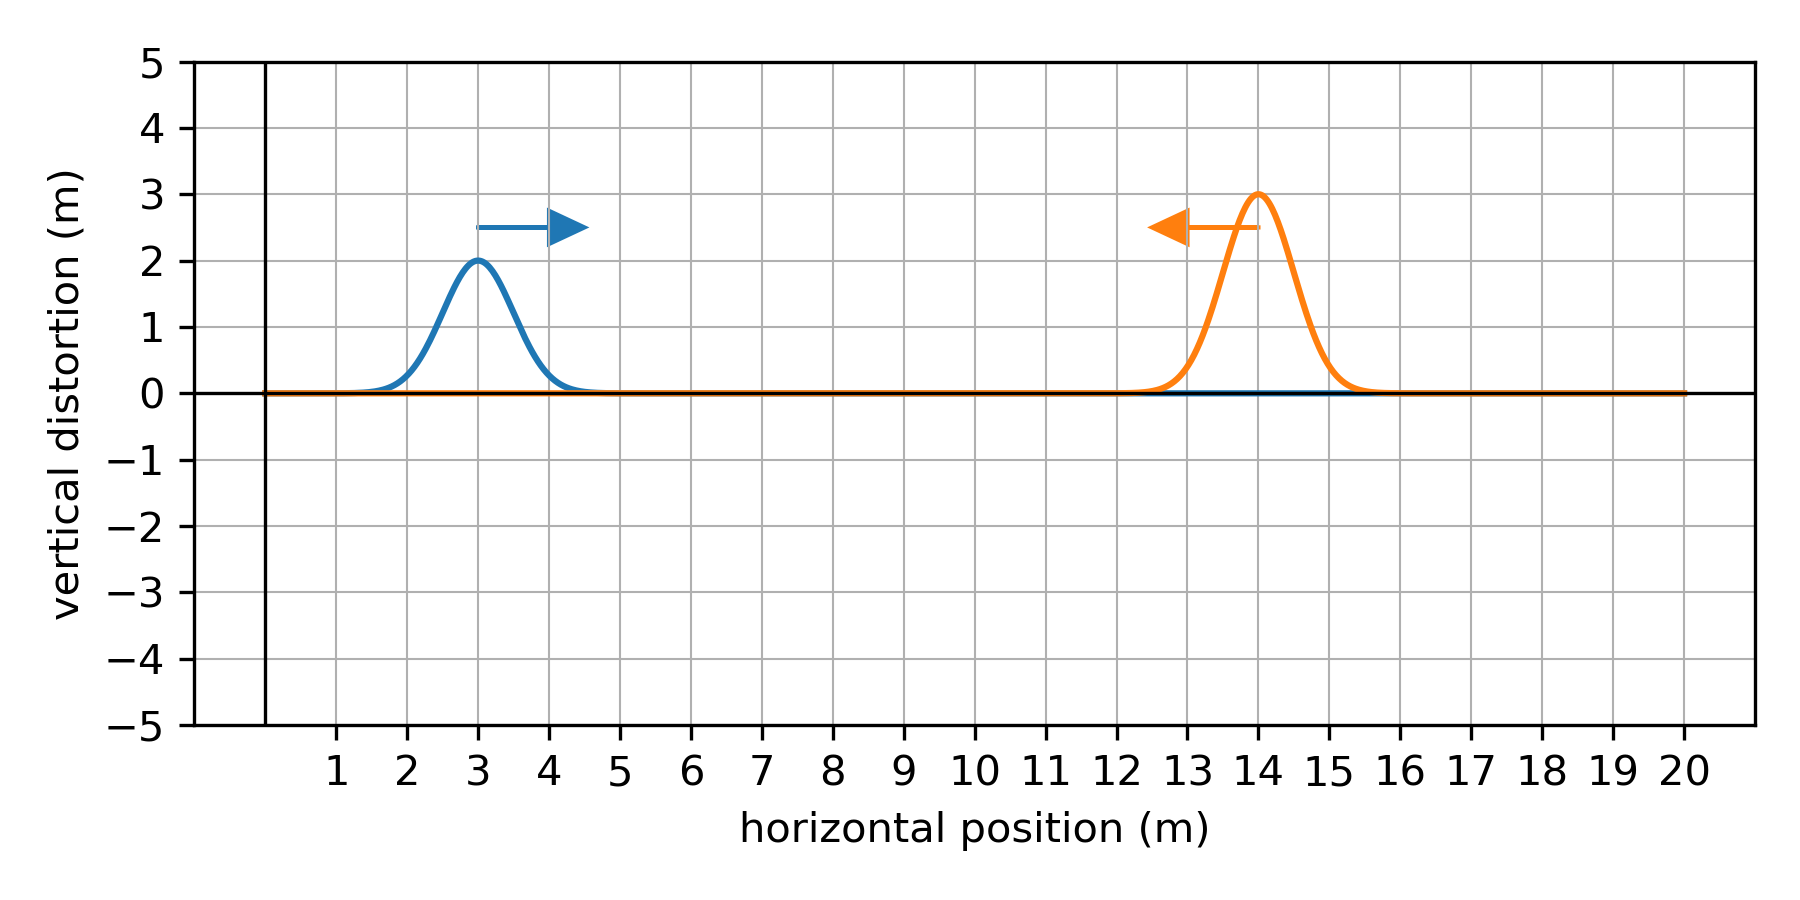
\includegraphics[scale=1]{week13-plot-upright-gauss-pulse.png}
	
	\item
	Again, two waves approach each other with speed $v=\SI{6}{m/s}$. At what time and where will these waves fully overlap and what will the wave look like at that time?\\
	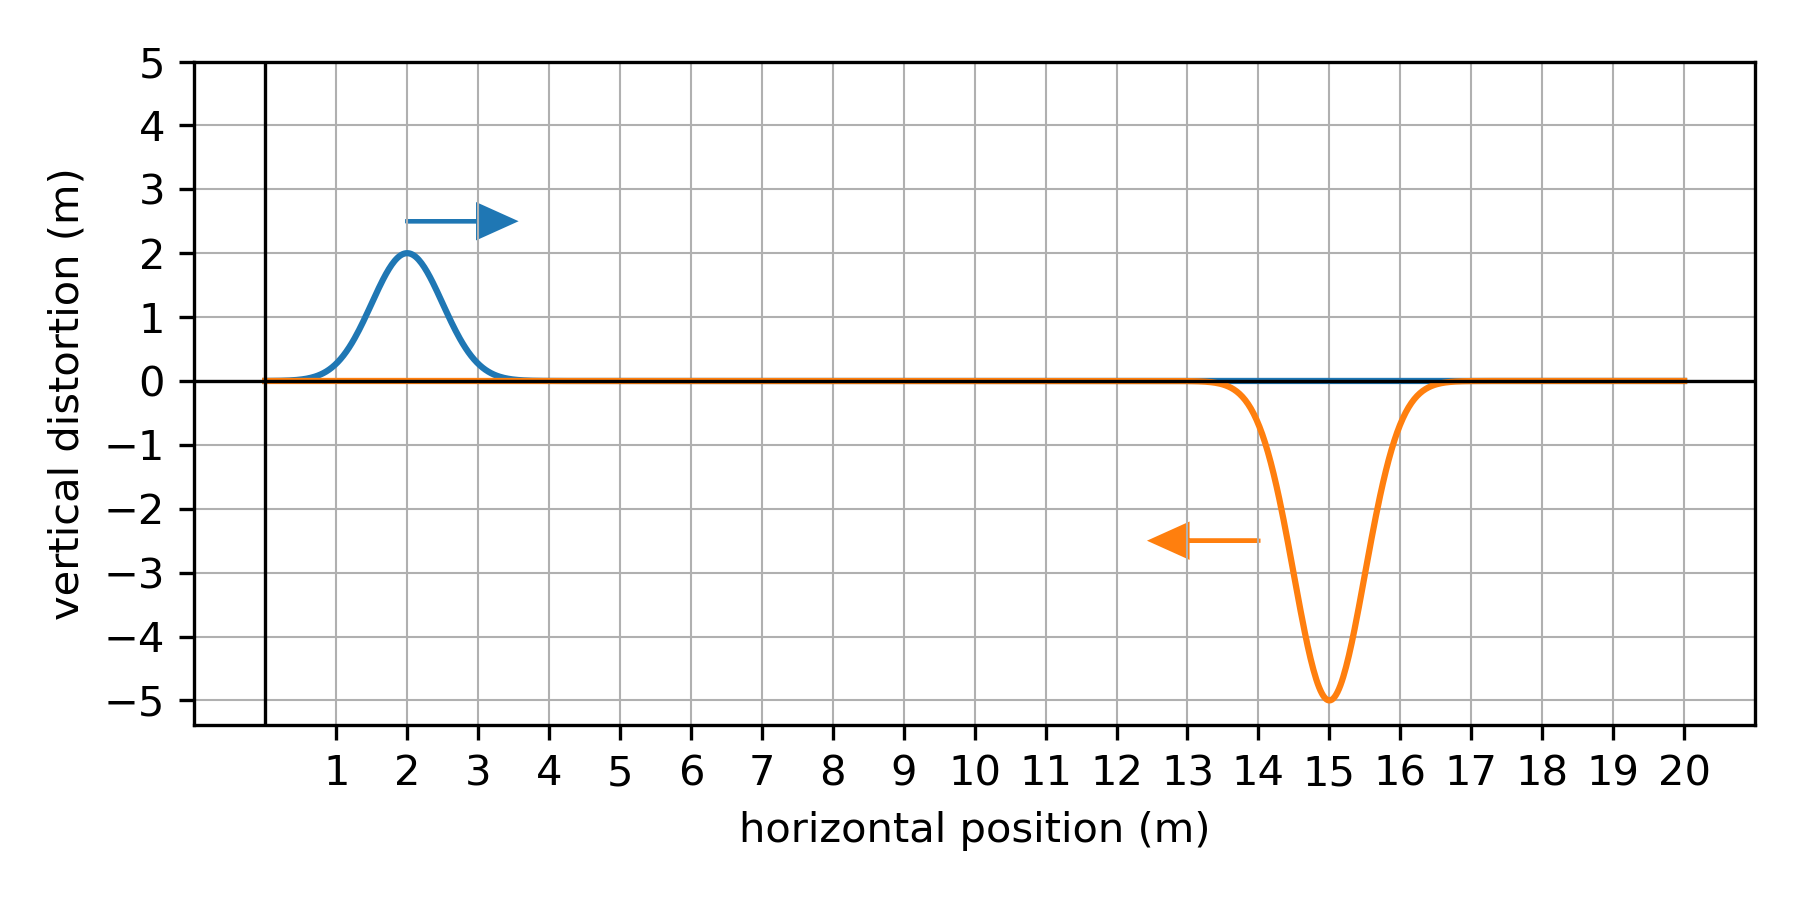
\includegraphics[scale=1]{week13-plot-invert-gauss-pulse.png}
	
	\vspace{-3cm}
	\item
	The plot below represents a standing wave in a string. How many antinodes are there? How many nodes are there? What is the wavelength of the string. If the speed of the wave on the string is $v=\SI{40}{m/s}$, then what input frequency produces this standing wave? What period of oscillation of the input frequency? \\
	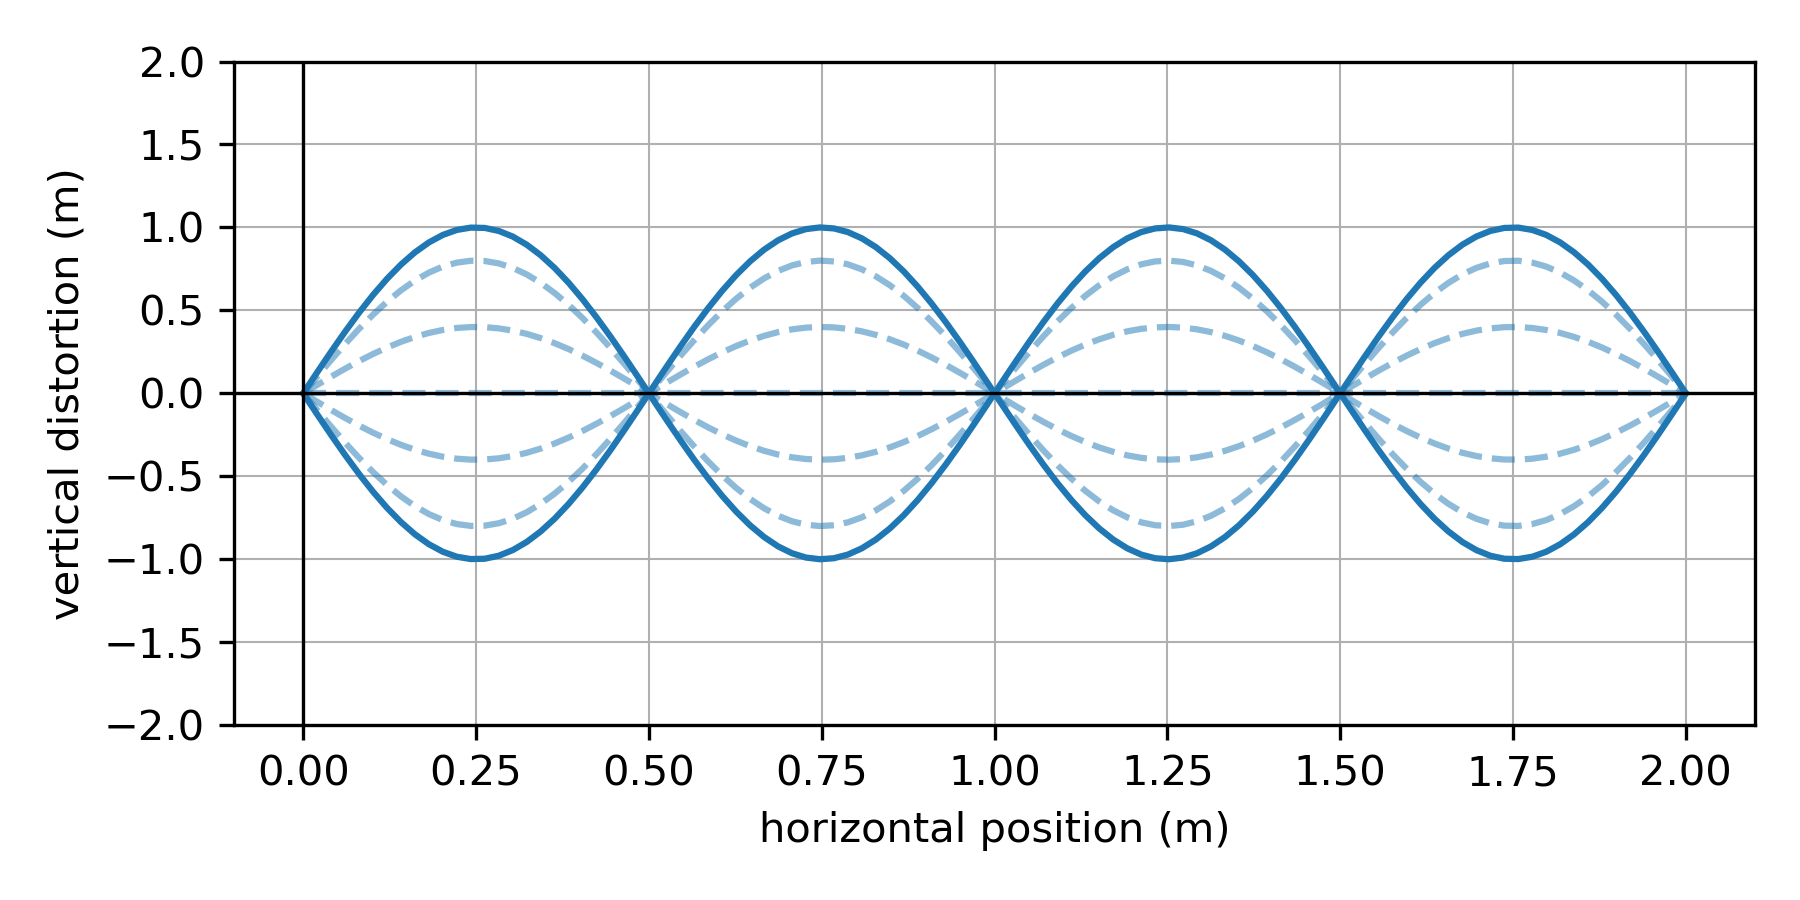
\includegraphics[scale=1]{week13-plot-standing-wave-1.png}
	
	\item
	If the string from the above problem has three antinodes, then what is the wavelength? If the velocity of the wave is still $v=\SI{40}{m/s}$, then what is the frequency? What is the wavelength and frequency when there are two antinodes? What about when there is one antinode? What is the fundamental frequency? What is the 10th harmonic frequency? What is the 10th harmonic wavelength?\bigskip
	
	\item
	Instead of changing the frequency to make a fewer anti-nodes, we could change the velocity instead, and the easiest way to do that is to adjust the force in the string. So if the standing wave goes from 4 antinodes to 3 antinodes, by what ratio does the \emph{speed} of the wave change? If the speed of the wave changes by this ratio, then by what ratio does the force on the string need to change? 
	
	\item
	Suppose a wave has a 4th harmonic frequency of \SI{200}{\hertz} then what is the fundamental frequency? 
	
	\item
	If a standing wave is produced a frequency of \SI{98}{\hertz} and a the next standing wave frequency is \SI{112}{\hertz}. What is the fundamental frequency and how many antinodes were there for these two standing waves?
	
	\item
	If you increase the tension in a string by a factor of 1.3, then by what factor do you change the fundamental frequency of a waves in that string? If you increase the tension in string by 10\%, then by what percent do you change the fundamental frequency?   
	
	

	
\end{enumerate}